\chapter{Quickstart}\indexmain{quickstart}\indexmain{example}

In this chapter we'll build a graph rewrite system from scratch.
We will use \GrG\ to construct non-deterministic state machines, and to remove $\varepsilon$-transitions from them.
This chapter gives a quick tour of \GrG\ and the process of using it; it esp. highlights its look and feel.
For comprehensive specifications, please take a look at the succeeding chapters.


%%%%%%%%%%%%%%%%%%%%%%%%%%%%%%%%%%%%%%%%%%%%%%%%%%%%%%%%%%%%%%%%%%%%%%%%%%%%%%%%%%%%%%%%%%%%%%%%
\section{Downloading \& Installing}

If you are reading this document, you probably have already downloaded the \GrG\ software from our website (\url{http://www.grgen.net}). Make sure you have the following system requirements installed and available in the search path:
\begin{itemize}
	\item Java 1.5 or above
	\item Mono 1.2.3 or above / Microsoft .NET 2.0 or above
\end{itemize}

\noindent{\bf If you're using Linux:}
Unpack the package to a directory of your choice, for example into \texttt{/opt/grgen}:
\begin{bash}
mkdir /opt/grgen
tar xvfj GrGenNET-V1_3_1-2007-12-06.tar.bz2
mv GrGenNET-V1_3_1-2007-12-06/* /opt/grgen/
rmdir GrGenNET-V1_3_1-2007-12-06
\end{bash}
Add the \texttt{/opt/grgen/bin} directory to your search paths, for instance if you use \texttt{bash} add a line to your \texttt{/home/.profile} file.
\begin{bash}
export PATH=/opt/grgen/bin:$PATH
\end{bash}
Furthermore we create a directory for our \GrG\ data, for instance by \texttt{mkdir /home/grgen}.

\vspace{2mm}
\noindent{\bf If you're using Microsoft Windows:}
Extract the .zip archive to a directory of your choice and add the \texttt{bin} subdirectory to your search path via \emph{control panel} $\rightarrow$ \emph{system properties} / environment variables.
Execute the \GrG\ assemblies from a command line window (\emph{Start} $\rightarrow$ \emph{Run...} $\rightarrow$ \texttt{cmd}).
For MS .NET the \texttt{mono} prefix is neither applicable nor needed.

\begin{note}
You might be interested in the syntax highlighting specifications of the \GrG-languages supplied for the vim, Emacs, and Notepad++ editors in the \texttt{syntaxhighlighting} subdirectory.
\end{note}


%%%%%%%%%%%%%%%%%%%%%%%%%%%%%%%%%%%%%%%%%%%%%%%%%%%%%%%%%%%%%%%%%%%%%%%%%%%%%%%%%%%%%%%%%%%%%%%%
\section{Creating a Graph Model}

In the directory \texttt{/home/grgen} we create a text file \texttt{StateMachine.gm} that contains the graph meta model for our state machine\footnote{You'll find the source code of this quick start example shipped with the \GrG\ package in the \texttt{examples/FiniteStateMachine/} directory.}.
By graph meta model we mean a set of node types and edge types which are available for building state machine graphs (see Chapter~
\ref{chapmodellang}).
Figure \ref{fig:quick:mm} shows the meta model.

\begin{figure}[htbp]
    \centering
    \begin{grgen}
node class State {
    id: int;
}

abstract node class SpecialState extends State;
node class StartState extends SpecialState;
node class FinalState extends SpecialState;
node class StartFinalState extends StartState, FinalState;

edge class Transition {
    Trigger: string;
}

const edge class EpsilonTransition extends Transition;
    \end{grgen}
    \caption{Meta Model for State Machines}
    \label{fig:quick:mm}
\end{figure}

What have we done?
We specified two base types, \texttt{State} for state nodes and \texttt{Transition} for transition edges that will connect the state nodes.
\texttt{State} has an integer attribute \texttt{id}, and \texttt{Transition} has a string attribute \texttt{Trigger} which indicates the character sequence for switching from the source state node to the destination state node.
The other types inherit from those base types (keyword \texttt{extends}). 
Inheritance works basically like inheritance in object oriented languages,
as does the \texttt{abstract} modifier for \texttt{SpecialState}, meaning that you cannot create a node of that precise type (only nodes of non-abstract subtypes).
With \texttt{StartFinalState} we have constructed a ``diamond'' type hierarchy,
highlighting the support for multiple inheritance.


%%%%%%%%%%%%%%%%%%%%%%%%%%%%%%%%%%%%%%%%%%%%%%%%%%%%%%%%%%%%%%%%%%%%%%%%%%%%%%%%%%%%%%%%%%%%%%%%
\section{Creating Graphs}
\label{sct:quick:create}

Let's test our graph meta model by creating a state machine graph.
We will use the \GrShell\ (see Chapter~\ref{chapgrshell}) and---for visualization---\yComp.
To get everything working we need a rule set file, too.
For the moment we just create an almost empty file \texttt{removeEpsilons.grg} in the \texttt{/home/grgen} directory, containing only the line
\begin{grgen}
#using "StateMachine.gm"
\end{grgen}
Now, we could start by launching the \GrShell\ and by typing the commands interactively.
However, in most of the cases this is not the preferred way, as we want to execute the same steps multiple times.
So instead, we create a \GrShell\ script \texttt{removeEpsilons.grs}, in the \texttt{/home/grgen} directory.
Figure \ref{fig:quick:shell} shows this script.
Run the script by executing \texttt{grshell removeEpsilons.grs}.
The first time you execute the script, it might take a while because \GrG\ has to compile the meta model and the rule set into .NET assemblies.

\begin{figure}[htbp]
    \centering
    \begin{grgen}
new graph removeEpsilons "StateMachineGraph"

new :StartState($=S, id=0)
new :FinalState($=F, id=3)
new :State($="1", id=1)
new :State($="2", id=2)
new @(S)-:Transition(Trigger="a")-> @("1")
new @("1")-:Transition(Trigger="b")-> @("2")
new @("2")-:Transition(Trigger="c")-> @(F)
new @(S)-:EpsilonTransition-> @("2")
new @("1")-:EpsilonTransition-> @(F)
new @(S)-:EpsilonTransition-> @(F)

show graph ycomp
    \end{grgen}
    \caption{Constructing a state machine graph in \GrShell}
    \label{fig:quick:shell}
\end{figure}

The graph viewer \yComp\ opens and after clicking the blue play ``layout graph'' button on the very right side of the button bar, you get a window similar to figure \ref{fig:quick:ycomp} (see also Section~\ref{tools:ycomp}).
Quit \yComp\ and exit the \GrShell\ by typing \texttt{exit}.

\begin{figure}[htbp]
	\centering
	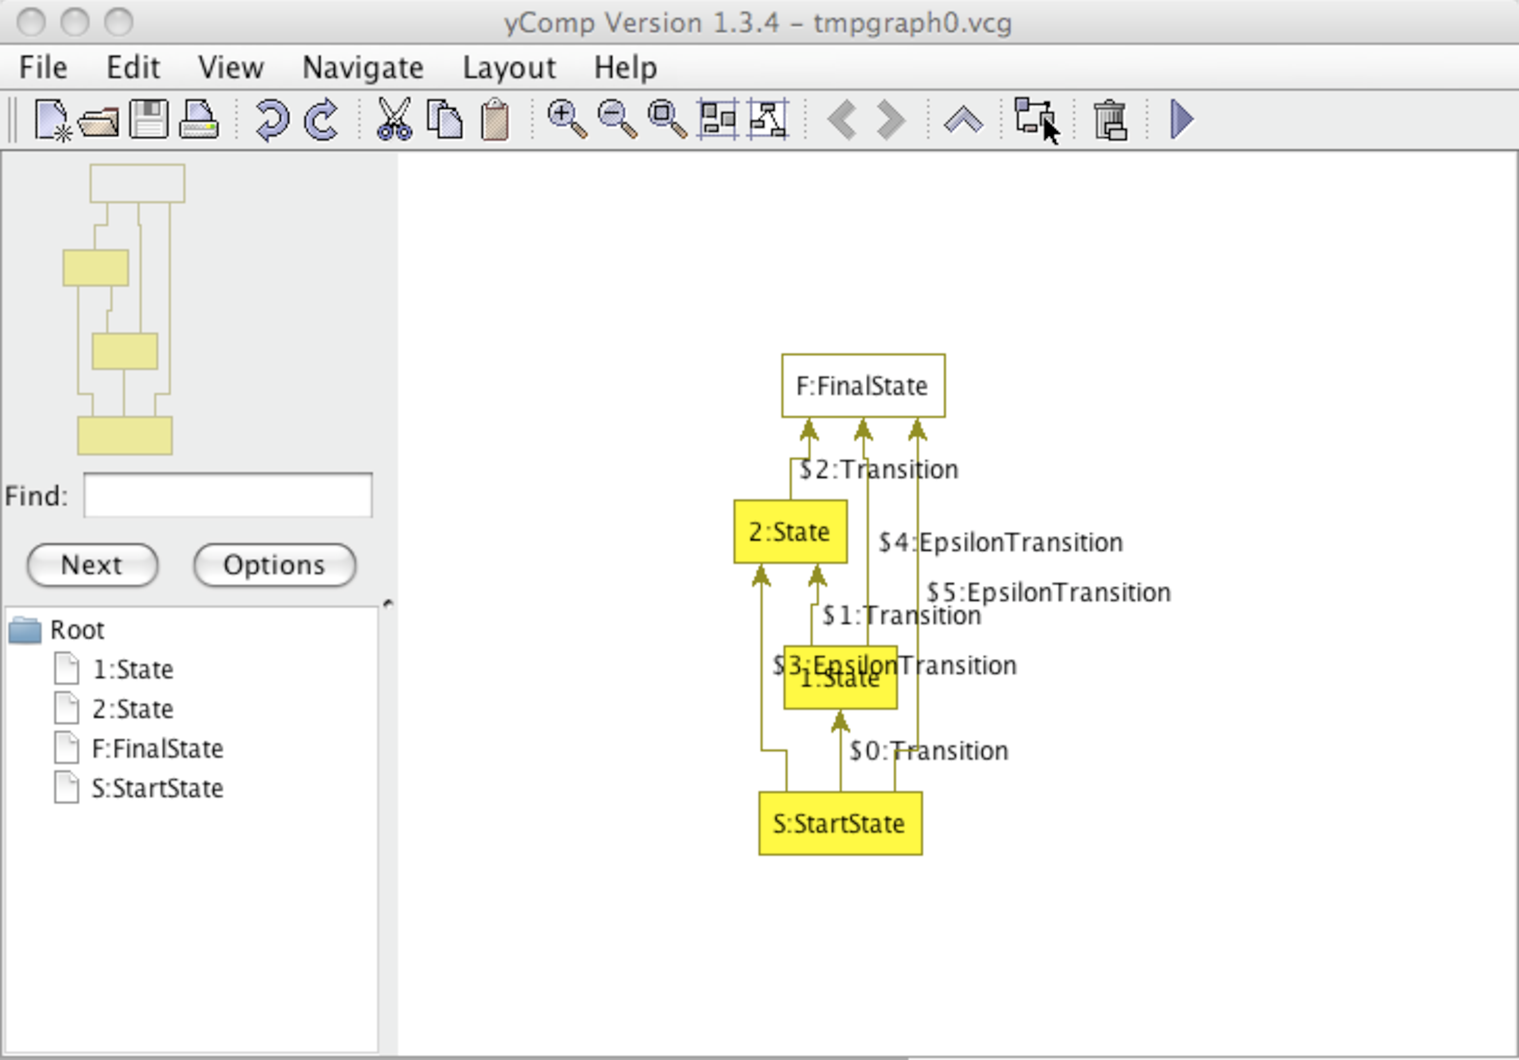
\includegraphics[width=0.99\linewidth]{fig/quickycomp}
	\caption{A first state machine (with $\varepsilon$-transitions)}
	\label{fig:quick:ycomp}
\end{figure}

Our script first creates an empty graph of the meta model \texttt{StateMachine} (which is referenced by the rule set \texttt{removeEpsilons.grg}) with the name \texttt{StateMachineGraph}.
Thereafter, it creates the nodes and edges, with a \texttt{name:type} colon notation -- the names are optional and missing here.
Note the inplace-arrow notation for edges (\texttt{-Edge->} resp.\ \texttt{-:EdgeType->}).
As you can see, attributes of graph elements can be set during creation with a call-like syntax.
The \texttt{\$} and \texttt{@} notation is due to the usage of \emph{persistent names}. 
Persistent names are set on creation by \texttt{\$=Identifier} and used later on by \texttt{@(Identifier)} to retrieve the graph element bound to them.
In addition to persistent names, another kind of ``names'' is available in the \GrShell\ with the \emph{global variables}, which would appear before the colon, but we did not use them in this script.
Persistent names must be identifier strings and not numbers, that's why we have to use the quote chars around \texttt{"1"} and \texttt{"2"}.

%%%%%%%%%%%%%%%%%%%%%%%%%%%%%%%%%%%%%%%%%%%%%%%%%%%%%%%%%%%%%%%%%%%%%%%%%%%%%%%%%%%%%%%%%%%%%%%%
\section{The Rewrite Rules}

We will now add the real rewrite rules to the rule set file \texttt{removeEpsilons.grg}.
The idea is to ``forward'' normal transitions over $\varepsilon$-transitions one after another, i.e.\ if we have a pattern like \texttt{a:State -:EpsilonTransition-> b:State -ne:Transition-> c:State} do we add another \texttt{a -ne-> c}.
After all transitions have been forwarded we can remove the $\varepsilon$-transitions alltogether.
The complete rule set is shown in figure \ref{fig:quick:ruleset}.
See Chapter~\ref{chaprulelang} for the rule set language reference.

\begin{figure}[htbp]
	\centering
	\begin{grgen}
#using "StateMachine.gm"

test checkStartState {
    x:StartState;
    negative {
        x;
        y:StartState;
    }
}

test checkDoublettes {
    negative {
        x:State -e:Transition-> y:State;
        hom(x,y);
        x -doublette:Transition-> y;
        if {typeof(doublette) == typeof(e);}
        if { ((typeof(e) == EpsilonTransition) || (e.Trigger == doublette.Trigger)); }
    }
}

rule forwardTransition {
    x:State -:EpsilonTransition-> y:State -e:Transition-> z:State;
    hom(x,y,z);
    negative {
        x -exists:Transition-> z;
        if {typeof(exists) == typeof(e);}
        if { ((typeof(e) == EpsilonTransition) || (e.Trigger == exists.Trigger)); }
    }
    modify {
        x -forward:typeof(e)-> z;
        eval {forward.Trigger = e.Trigger;}
    }
}

rule addStartFinalState {
    x:StartState -:EpsilonTransition-> :FinalState;
    modify {
        y:StartFinalState<x>;
        emit("Start state (", x.id, ") mutated into a start-and-final state");
    }
}

rule addFinalState {
    x:State -:EpsilonTransition-> :FinalState;
    if {typeof(x) < SpecialState;}
    modify {
        y:FinalState<x>;
    }
}

rule removeEpsilonTransition {
    -:EpsilonTransition->;
    replace {}
}
	\end{grgen}
	\caption{Rule set for removing $\varepsilon$-transitions}
	\label{fig:quick:ruleset}
\end{figure}

Let's inspect the rule set specification in detail: The rule set file consists of a number of \texttt{rule}s and \texttt{test}s, each of them bearing a name, like \texttt{forwardTransition}.
Rules contain a pattern specified by semicolon-terminated graphlets, and a rewrite part given with a nested modify or replace block.
Tests contain only a pattern; they are used to check for a certain pattern without doing any rewrite operations.
If a rule is applied, \GrG\ tries to find the pattern within the host graph, for instance within the graph we created in Section~\ref{sct:quick:create}.
Of course there could be several matches for a pattern---\GrG\ will choose one of them arbitrarily (technically the first match in an implementation defined order).

Figure \ref{fig:quick:ruleset} also displays the syntax \texttt{name:NodeType} for nodes and \texttt{-name:EdgeType->} for Edges, which we have already seen in Section~\ref{sct:quick:create}, again with an optional name.
But here the meaning of a \emph{declaration} \texttt{name:Type} depends on whether it appears in the pattern or the rewrite part.
A declaration in the pattern defines a pattern element that is to be bound by searching, resp. matching in the host graph, whereas a declaration in the rewrite part defines an element that is to be created (so only the latter does the same as its counterpart from the shell script).
An element with a name assigned to can be \emph{referenced} from another graphlet, or from the rewrite block, by noting down simply the name for a node, or using the syntax \texttt{-name->} for an edge (a name can be referenced in the same or nested blocks).
If you want to ``do something'' with your specified graph element ``in another location'' (which may mean simply linking a node to another edge), define a name; otherwise an anonymous graph element will work fine (like the \texttt{:FinalState} or \texttt{-:EpsilonTransistion->} declarations that will be bound to a node of type \texttt{FinalState} resp.\ an edge of type \texttt{EpsilonTransition}, but are inaccessible for other operations) .
Also have a look at example \ref{ex:somegraphlets} on page \pageref{ex:somegraphlets} for additional pattern specifications.

The rewrite part can be given in one of two modes, \texttt{modify} mode or \texttt{replace} mode.
In replace mode, every graph element of the pattern which is not referenced within the \texttt{replace} block is deleted.
The modify mode, in contrast, deletes nothing (by default), but just adds or keeps graph elements.
Instead, the modify part allows for \emph{explicit} deletion of graph elements by using a \texttt{delete} command inside the \texttt{modify} block.

What else do we use?
We employ \texttt{negative} patterns; they prevent their containing rule from getting applied if the negative pattern is found.
We also use attribute conditions noted down inside an \texttt{if \{\dots\}} to express non-structural constraints; a rule is only applicable if all such conditions are evaluated to true.
Attributes of graph elements are accessed with dot notation (as in \texttt{e.Trigger}).
The \texttt{hom(x,y)} and \texttt{hom(x,y,z)} statements mean ``match the embraced nodes homomorphically'', i.e.\ they can (but don't have to) be matched to the same node within the host graph.

The \texttt{eval \{\dots\}} statement in the rewrite part is used to evaluate or recalculate attributes of graph elements.
The \texttt{emit} statement prints a string to \texttt{stdout}.
Have a look at the statement \texttt{y:StartFinalState<x>} in \texttt{addStartFinalState}: we \emph{retype} the node \texttt{x}.
That means that the newly created node \texttt{y} can be found at the position of \texttt{x} in the graph, that it bears its persistent name, and that the attributes common to the new and the previous type keep their old values -- only the node type is  changed or casted to \texttt{StartFinalState}.


%%%%%%%%%%%%%%%%%%%%%%%%%%%%%%%%%%%%%%%%%%%%%%%%%%%%%%%%%%%%%%%%%%%%%%%%%%%%%%%%%%%%%%%%%%%%%%%%
\section{Applying the Rules}

The created rewrite rules are transformation primitives, we must compose them in order to implement more complex functionality.
For instance we don't want to forward just one $\varepsilon$-transition as \texttt{forwardTransition} would do; we want to forward them all.
Such a rule composition is called a \emph{graph rewrite sequence} (see Chapter~\ref{cha:xgrs}).
We add the following line to our shell script \texttt{removeEpsilons.grs}:

\begin{grgen}
debug exec checkStartState && !checkDoublettes && (forwardTransition* | addStartFinalState | addFinalState* | removeEpsilonTransition* | true)
\end{grgen}

This looks like a boolean expression and in fact it behaves similarly.
The whole expression is evaluated from left to right.
A rule is successfully evaluated if a match could be found (and is rewritten, but this won't change the execution result).
The negation operator \texttt{!} just toggles the result.
We first check for a valid state machine, i.e.\ if the host graph contains exactly one start state and no redundant transitions.
Thereafter we do the actual rewriting.
These three steps are connected by lazy-evaluation-ands (\texttt{\&\&}), i.e.\ if one of them fails the evaluation will be canceled.
We continue with disjunctively connected rules (by \texttt{|}).
The eager operator causes all rules to get executed, but only one must find a match to count as a success; the final \texttt{true} ensures overall success.
The \texttt{*} is used to apply the rule repeatedly as long as a match can be found.
This includes applying the rule zero times.
Even in this case \texttt{Rule*} is still successful.


%%%%%%%%%%%%%%%%%%%%%%%%%%%%%%%%%%%%%%%%%%%%%%%%%%%%%%%%%%%%%%%%%%%%%%%%%%%%%%%%%%%%%%%%%%%%%%%%
\section{Debugging and Output}

If you execute the modified \GrShell\ script, \GrG\ starts its debugger.
This way you can follow the execution of the graph rewrite sequence step by step in \yComp.
Just play around with the keys \texttt{d}, \texttt{s}, and \texttt{r} in \GrShell: the \texttt{d} key lets you follow a single rule application in a matching and a rewriting step, highlighting the found spot in the graph; the \texttt{s} key jumps to the next rule; and the \texttt{r} key runs to the end of the graph rewrite sequence.
After sequence execution, you should see a graph like the one in Figure \ref{fig:quick:final}.

\begin{figure}[htbp]
	\centering
	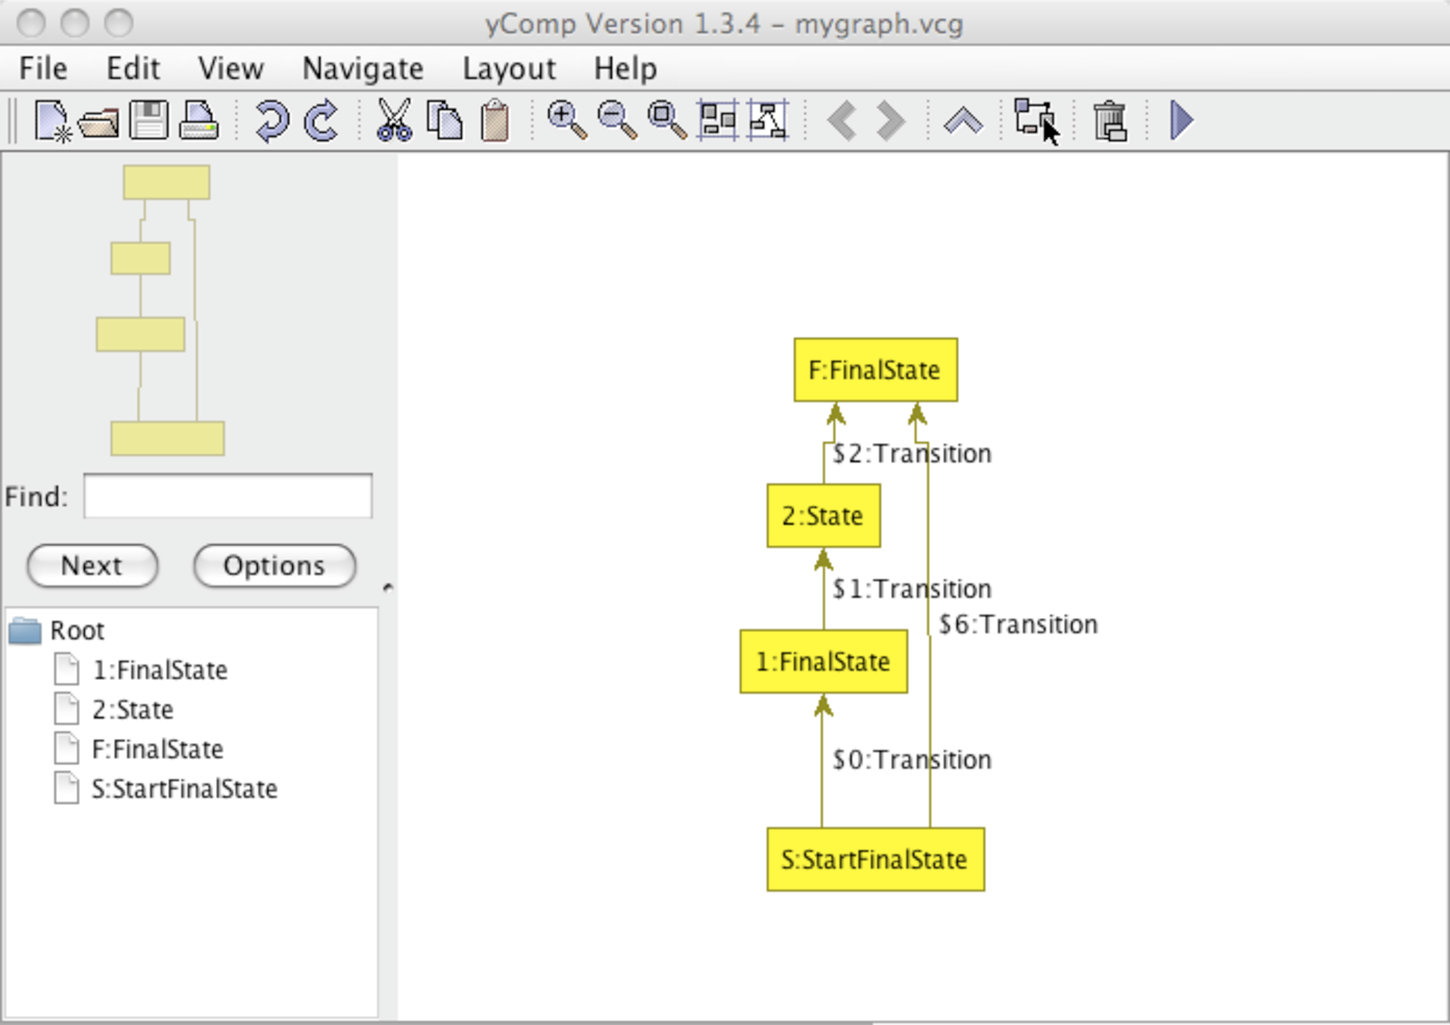
\includegraphics[width=0.99\linewidth]{fig/quickfinal}
	\caption{A state machine without $\varepsilon$-transitions}
	\label{fig:quick:final}
\end{figure}

If everything is working fine you can delete the \texttt{debug} keyword in front of the \texttt{exec} and just (re)use this sequence as you need to.
Maybe you want to save a visualization of the resulting graph.
This is possible by typing \texttt{dump graph mygraph.vcg} in \GrShell,
which is then writing \texttt{mygraph.vcg} into the current directory in the VCG format readable by \yComp.
Or you want to save the resulting graph as such, to continue processing later on.
Say \texttt{export mygraph.grs} in \GrShell\ then, it will write a file composed of \texttt{new} commands as is our input file from Figure \ref{fig:quick:shell}, but containing the $\varepsilon$-free graph.

Feel free to browse the \texttt{examples} folder shiped with \GrG;
have a look at the succession of examples in the \texttt{FiniteStateMachine} and \texttt{ProgramGraphs} subfolders,
they give an overview over most of the capabilities of the software.

